\documentclass[10pt,a4paper]{article}

% ==============================================================================
% EXPERIMENT 04: HC-SR04 ULTRASONIC SENSOR & ARDUINO UNO
% Comprehensive Practical Lab Copy & Technical Manual (Exact 4-Page Master Edition)
% Department of Computer Science & Engineering / Information Technology
% ==============================================================================
\usepackage[utf8]{inputenc}
\usepackage[T1]{fontenc}
\usepackage{lmodern}
\usepackage[left=1.5cm, right=1.5cm, top=1.2cm, bottom=1.2cm]{geometry}
\usepackage{amsmath,amssymb,amsfonts,amsthm}
\usepackage{graphicx}
\usepackage{tikz}
\usetikzlibrary{arrows.meta,positioning,shapes.geometric,decorations.pathreplacing,calc}
\usepackage{circuitikz}
\usepackage{listings}
\usepackage{tcolorbox}
\tcbuselibrary{skins,breakable}
\usepackage{booktabs}
\usepackage{tabularx}
\usepackage{array}
\usepackage{titlesec}
\usepackage{enumitem}
\usepackage{caption}
\usepackage{microtype}
\usepackage{float}
\usepackage{hyperref}

\pagestyle{plain}

\hypersetup{
    hidelinks,
    pdfauthor={Department of Computer Science and Engineering},
    pdftitle={Experiment 04: HC-SR04 Ultrasonic Distance Sensor Interfacing with Arduino UNO},
    pdfsubject={IoT Laboratory Practical Record - Ultrasonic Acoustic Ranging and Telemetry}
}

% Section Heading Formatting
\titleformat{\section}
  {\normalfont\normalsize\bfseries}{\thesection}{0.8em}{}[\titlerule]
\titleformat{\subsection}
  {\normalfont\small\bfseries}{\thesubsection}{0.5em}{}
\titleformat{\subsubsection}
  {\normalfont\footnotesize\bfseries\itshape}{\thesubsubsection}{0.4em}{}

\titlespacing*{\section}{0pt}{4pt}{2pt}
\titlespacing*{\subsection}{0pt}{3pt}{1pt}
\titlespacing*{\subsubsection}{0pt}{2pt}{1pt}

\setlist{itemsep=0.5pt, parsep=0pt, topsep=1.0pt, partopsep=0pt}
\setlength{\parskip}{0pt}
\setlength{\parsep}{0pt}
\setlength{\headsep}{0pt}
\setlength{\topskip}{0pt}

% Code Listing Styling (Strict Monochrome)
\lstdefinestyle{bwArduino}{
    language=C++,
    basicstyle=\ttfamily\scriptsize,
    keywordstyle=\bfseries,
    commentstyle=\itshape,
    stringstyle=\ttfamily,
    numbers=left,
    numberstyle=\tiny,
    numbersep=4pt,
    stepnumber=1,
    breaklines=true,
    breakatwhitespace=true,
    frame=single,
    rulecolor=\color{black},
    tabsize=2,
    showstringspaces=false,
    columns=fullflexible,
    keepspaces=true,
    lineskip=-0.2pt,
    aboveskip=2pt,
    belowskip=2pt
}

\lstdefinestyle{bwTerminal}{
    basicstyle=\ttfamily\scriptsize,
    numbers=none,
    breaklines=true,
    breakatwhitespace=true,
    frame=single,
    rulecolor=\color{black},
    columns=fullflexible,
    keepspaces=true,
    lineskip=0.0pt,
    aboveskip=2pt,
    belowskip=2pt
}

\captionsetup{font=footnotesize,labelfont=bf,skip=2pt}

\begin{document}

% ==============================================================================
% PAGE 1: HEADER, AIM, APPARATUS & THEORETICAL FOUNDATIONS
% ==============================================================================
\begin{center}
    {\Large\bfseries INTERNET OF THINGS (IoT) LABORATORY}\\[0.05cm]
    {\large\bfseries PRACTICAL EXPERIMENT RECORD}\\[0.06cm]
    {\footnotesize\textbf{Department of Computer Science and Engineering / Information Technology}}\\[0.02cm]
    {\scriptsize\textbf{Academic Session: 2025--2026 \quad $\bullet$ \quad Degree: Bachelor of Technology (B.Tech)}}
\end{center}
\vspace{-0.32cm}
\rule{\textwidth}{0.8pt}
\vspace{0.08cm}

\begin{center}
    {\large\bfseries Experiment 04: Interfacing HC-SR04 Ultrasonic Sensor with Arduino UNO}\\[0.04cm]
    {\small\textbf{Non-Contact Acoustic Distance Measurement, Time-of-Flight Physics \& Serial Telemetry}}
\end{center}
\vspace{-0.18cm}
\noindent\footnotesize\textbf{Course Code:} PCC-CS791 / IT-LAB \hfill \textbf{Semester:} VI / VII \hfill \textbf{Date of Experiment:} 26/08/2026
\vspace{0.02cm}
\hrule
\vspace{0.10cm}

\section*{1. Aim \& Objectives}
\begin{itemize}[noitemsep]
    \item To interface the HC-SR04 ultrasonic distance sensor module with the Arduino UNO development board (ATmega328P MCU).
    \item To study the fundamental physical principles of electro-acoustic transducers, piezoelectric excitation, and Time-of-Flight (ToF).
    \item To generate a precision microsecond trigger pulse ($10\,\mu\text{s}$) on GPIO Pin D8 and capture the echo response duration on GPIO Pin D7.
    \item To mathematically derive distance using the velocity of sound in air ($v \approx 343\,\text{m/s}$ at $20^\circ\text{C}$, giving $0.03434\,\text{cm}/\mu\text{s}$).
    \item To stream continuous real-time distance telemetry over the UART serial interface at 9600 Baud to the host workstation.
    \item To analyze spatial beam dispersion ($15^\circ$), surface acoustic absorption, and minimum/maximum ranging limits ($2\,\text{cm} - 400\,\text{cm}$).
\end{itemize}

\section*{2. Hardware Apparatus Required \& Specifications}
\begin{table}[H]
\centering
\footnotesize
\renewcommand{\arraystretch}{1.15}
\begin{tabularx}{\textwidth}{|c|l|X|c|}
\hline
\textbf{S.No.} & \textbf{Component Name} & \textbf{Technical Specifications / Parametric Values} & \textbf{Quantity} \\
\hline
1 & Arduino UNO R3 & ATmega328P 8-bit AVR RISC MCU, 16 MHz Crystal, 5V Operating Logic & 1 unit \\
2 & HC-SR04 Sensor & Ultrasonic Transceiver, $40\,\text{kHz}$ Frequency, Range: $2\,\text{cm} - 400\,\text{cm}$, Resolution: $0.3\,\text{cm}$ & 1 unit \\
3 & Solderless Breadboard & Standard 830 Tie-Point Breadboard with Dual Power Distribution Rails & 1 unit \\
4 & Jumper Wires & 24 AWG Solid-Core Male-to-Male Interconnect Connecting Wires & 4 units \\
5 & USB Cable & USB Type-A to Type-B Data and Power Cable & 1 unit \\
6 & Target Obstacle / Metric Rule & Flat acoustic reflective planar surface (cardboard/notebook) and metric scale & 1 set \\
\hline
\end{tabularx}
\caption{\textbf{Hardware Components and Technical Specifications for Experiment 04.}}
\end{table}

\section*{3. Theoretical Background \& Working Principle}

\subsection*{A. Definition \& Physics of Ultrasonic Sensor}
An \textbf{Ultrasonic Sensor} is an active electro-acoustic transducer that detects the presence of objects and measures physical distances by emitting high-frequency ultrasonic acoustic waves (typically $40\,\text{kHz}$, well beyond human audible perception, $\approx 20\,\text{kHz}$) and detecting the reflected acoustic pressure wave. The sensor operates via the \textbf{Piezoelectric Effect}:
\begin{itemize}[noitemsep]
    \item \textbf{Inverse Piezoelectric Effect (Transmitter `T`):} When an alternating voltage is applied across a piezoelectric ceramic crystal (Lead Zirconate Titanate, PZT), the crystal lattice vibrates at its resonant frequency ($40\,\text{kHz}$), emitting longitudinal acoustic waves.
    \item \textbf{Direct Piezoelectric Effect (Receiver `R`):} When the reflected acoustic wave strikes the receiver crystal, mechanical compression induces a proportional electrical charge, generating a microvolt signal that is amplified by an internal operational amplifier.
\end{itemize}

\subsection*{B. Operational Working Principle of HC-SR04 Module}
The HC-SR04 module features four external terminals: $V_{CC}$ ($+5\,\text{V}$ DC), $\text{GND}$ ($0\,\text{V}$), $\text{TRIG}$ (Trigger Input), and $\text{ECHO}$ (Echo Output). The measurement sequence executes in four discrete phases:
\begin{enumerate}[leftmargin=*]
    \item \textbf{Trigger Signal Generation:} The host microcontroller drives `TRIG` HIGH for a minimum of $10\,\mu\text{s}$ ($T_{\text{trig}} \ge 10\,\mu\text{s}$), initiating the internal measurement cycle.
    \item \textbf{Sonic Burst Emission:} The sensor's onboard controller automatically generates an 8-cycle burst of $40\,\text{kHz}$ square waves to excite `T`.
    \item \textbf{Echo Pulse Width Assertion:} Simultaneously with sound emission, the sensor drives its `ECHO` output pin to logic HIGH ($+5\,\text{V}$).
    \item \textbf{Echo Reception \& Return to Low:} When the emitted acoustic wave reflects off an obstacle and strikes receiver `R`, the internal comparator drives `ECHO` back to logic LOW ($0\,\text{V}$). The HIGH duration $\Delta t$ corresponds to two-way Time-of-Flight (ToF).
\end{enumerate}

\newpage

% ==============================================================================
% PAGE 2: MATHEMATICAL DERIVATIONS & CIRCUIT SCHEMATICS
% ==============================================================================
\subsection*{C. Mathematical Derivation of Distance}
Let $d$ be the one-way distance between the sensor and the target obstacle, and let $\Delta t$ be the measured duration of the HIGH state on the `ECHO` pin. Because the acoustic pulse travels to the object and reflects back, the total distance traversed by the wave is $2d$.

Applying the classical kinematic equation of motion:
\begin{equation}
\text{Total Distance} = 2 \cdot d = v \cdot \Delta t \implies d = \frac{v \cdot \Delta t}{2}
\end{equation}
Where $v$ is the velocity of sound in dry air.

\subsubsection*{1. Speed of Sound Temperature Dependency}
The velocity of sound in an ideal gas medium depends on thermodynamic temperature according to Laplace's equation:
\begin{equation}
v(T) = \sqrt{\frac{\gamma \cdot R \cdot T_K}{M}} = 331.3 \cdot \sqrt{1 + \frac{T_C}{273.15}} \approx 331.3 + (0.606 \cdot T_C)\;\text{m/s}
\end{equation}
At standard laboratory temperature ($T_C = 20^\circ\text{C}$):
\begin{equation}
v(20^\circ\text{C}) \approx 331.3 + (0.606 \times 20) = 343.42\,\text{m/s} = 0.03434\,\text{cm}/\mu\text{s} = \frac{1}{29.12}\,\text{cm}/\mu\text{s}
\end{equation}

\subsubsection*{2. Distance Calculation Formula in Centimeters}
Substituting the velocity into the two-way distance derivation:
\begin{equation}
d\,(\text{cm}) = \frac{\Delta t\,(\mu\text{s}) \times 0.03434\,\text{cm}/\mu\text{s}}{2} = \frac{\Delta t\,(\mu\text{s})}{58.24} \approx \frac{\Delta t \times 0.034}{2}
\end{equation}
Thus, for every $58.24\,\mu\text{s}$ of measured echo pulse width, the obstacle is positioned exactly $1.0\,\text{cm}$ away.

\section*{4. Circuit Schematic, Wiring Matrix \& Timing Waveforms}

\subsection*{A. Hardware Pin Interconnection Matrix}
\begin{table}[H]
\centering
\footnotesize
\renewcommand{\arraystretch}{1.15}
\begin{tabularx}{\textwidth}{|l|l|l|X|}
\hline
\textbf{Arduino UNO Pin} & \textbf{HC-SR04 Terminal} & \textbf{Pin Label} & \textbf{Functional Description \& Logic Level} \\
\hline
$+5\text{V}$ Power Pin & Pin 1 (VCC) & $V_{CC}$ & $+5.0\,\text{V}$ DC Regulated Power Supply ($I_{\text{active}} \approx 15\,\text{mA}$) \\
Digital Pin 8 (D8) & Pin 2 (TRIG) & Trigger & Microcontroller Output: $10\,\mu\text{s}$ Active-HIGH Start Trigger Pulse \\
Digital Pin 7 (D7) & Pin 3 (ECHO) & Echo & Microcontroller Input: Active-HIGH Pulse ($T_{\text{high}} = \text{ToF}$) \\
GND Power Pin & Pin 4 (GND) & Ground & Common System Ground Return Path ($0.0\,\text{V}$) \\
\hline
\end{tabularx}
\caption{\textbf{Table 4.1: Pin Mapping Table between Arduino UNO and HC-SR04 Module.}}
\end{table}

\subsection*{B. CircuiTikZ Hardware Interfacing Schematic}
\begin{figure}[H]
\centering
\begin{circuitikz}[scale=0.82, every node/.style={transform shape}]
    % Arduino Board Block
    \draw[thick, fill=white] (0, 0) rectangle (4.6, 3.8);
    \node at (2.3, 3.45) {\textbf{\large Arduino UNO R3}};
    \node at (2.3, 3.05) {\footnotesize (ATmega328P MCU)};

    % Arduino Pin Nodes
    \node[anchor=west] at (0.3, 2.4) {\textbf{5V} (Power)};
    \node[anchor=west] at (0.3, 1.7) {\textbf{D8} (Trigger Pin)};
    \node[anchor=west] at (0.3, 1.0) {\textbf{D7} (Echo Pin)};
    \node[anchor=west] at (0.3, 0.3) {\textbf{GND} (Ground)};

    % HC-SR04 Module Block
    \draw[thick, fill=white] (10.0, 0) rectangle (16.2, 3.8);
    \node at (13.1, 3.45) {\textbf{\large HC-SR04 Module}};
    \node at (13.1, 3.05) {\footnotesize (Ultrasonic Transceiver)};

    % Transducer circles on sensor
    \draw[thick, fill=white] (13.8, 1.9) circle (0.50cm);
    \node at (13.8, 1.9) {\textbf{\small T}};
    \node at (13.8, 1.15) {\tiny Transmitter};

    \draw[thick, fill=white] (15.3, 1.9) circle (0.50cm);
    \node at (15.3, 1.9) {\textbf{\small R}};
    \node at (15.3, 1.15) {\tiny Receiver};

    % HC-SR04 Pin Labels (Left edge of sensor)
    \node[anchor=west] at (10.1, 2.4) {\textbf{VCC} (Pin 1)};
    \node[anchor=west] at (10.1, 1.7) {\textbf{TRIG} (Pin 2)};
    \node[anchor=west] at (10.1, 1.0) {\textbf{ECHO} (Pin 3)};
    \node[anchor=west] at (10.1, 0.3) {\textbf{GND} (Pin 4)};

    % Straight Connecting Wires
    \draw[thick, -{Stealth[length=2.5mm]}] (4.6, 2.4) -- (10.0, 2.4);
    \node[above, font=\scriptsize] at (7.3, 2.4) {$+5\text{V DC Regulated Power}$};

    \draw[thick, -{Stealth[length=2.5mm]}] (4.6, 1.7) -- (10.0, 1.7);
    \node[above, font=\scriptsize] at (7.3, 1.7) {Trigger Output ($10\,\mu\text{s}$ Pulse)};

    \draw[thick, {Stealth[length=2.5mm]}-] (4.6, 1.0) -- (10.0, 1.0);
    \node[above, font=\scriptsize] at (7.3, 1.0) {Echo Input ($\text{Pulse Width } \Delta t$)};

    \draw[thick, -{Stealth[length=2.5mm]}] (4.6, 0.3) -- (10.0, 0.3);
    \node[above, font=\scriptsize] at (7.3, 0.3) {Common Ground ($0\text{V}$)};
\end{circuitikz}
\caption{\textbf{Figure 4.1: Interfacing Schematic of HC-SR04 Ultrasonic Sensor with Arduino UNO.}}
\end{figure}

\subsection*{C. Time-of-Flight Acoustic Timing Waveform}
\begin{figure}[H]
\centering
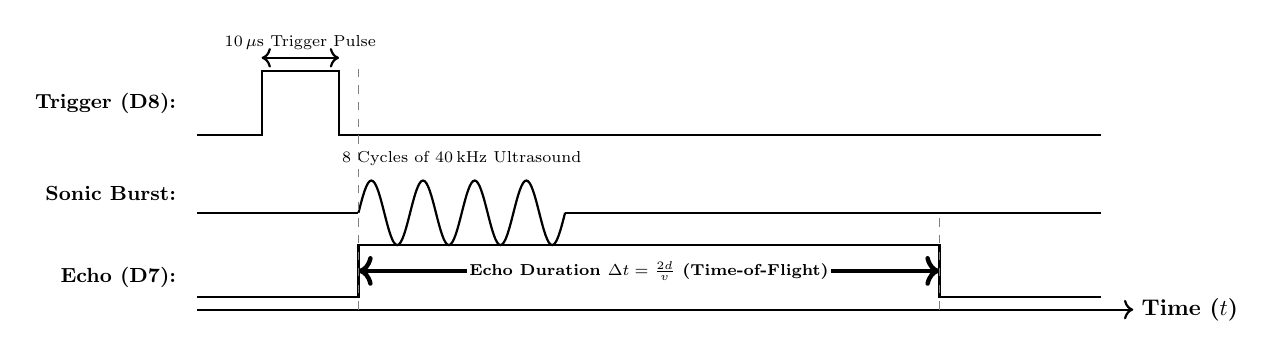
\begin{tikzpicture}[scale=0.82, every node/.style={transform shape}]
    % Time axis line
    \draw[->, thick] (0,0) -- (14.5,0) node[right] {\textbf{Time ($t$)}};

    % Signal 1: Trigger Pulse
    \node[anchor=east, font=\small\bfseries] at (-0.2, 3.2) {Trigger (D8):};
    \draw[thick] (0, 2.7) -- (1.0, 2.7) -- (1.0, 3.7) -- (2.2, 3.7) -- (2.2, 2.7) -- (14.0, 2.7);
    \draw[<->, thick] (1.0, 3.9) -- (2.2, 3.9) node[midway, above, font=\scriptsize] {$10\,\mu\text{s}$ Trigger Pulse};

    % Signal 2: Ultrasonic 40kHz Burst
    \node[anchor=east, font=\small\bfseries] at (-0.2, 1.8) {Sonic Burst:};
    \draw[thick] (0, 1.5) -- (2.5, 1.5);
    % 8 cycle bursts
    \draw[thick] (2.5, 1.5) sin (2.7, 2.0) cos (2.9, 1.5) sin (3.1, 1.0) cos (3.3, 1.5)
                            sin (3.5, 2.0) cos (3.7, 1.5) sin (3.9, 1.0) cos (4.1, 1.5)
                            sin (4.3, 2.0) cos (4.5, 1.5) sin (4.7, 1.0) cos (4.9, 1.5)
                            sin (5.1, 2.0) cos (5.3, 1.5) sin (5.5, 1.0) cos (5.7, 1.5);
    \draw[thick] (5.7, 1.5) -- (14.0, 1.5);
    \node[above, font=\scriptsize] at (4.1, 2.1) {8 Cycles of $40\,\text{kHz}$ Ultrasound};

    % Signal 3: Echo Output
    \node[anchor=east, font=\small\bfseries] at (-0.2, 0.5) {Echo (D7):};
    \draw[thick] (0, 0.2) -- (2.5, 0.2) -- (2.5, 1.0) -- (11.5, 1.0) -- (11.5, 0.2) -- (14.0, 0.2);
    \draw[<->, ultra thick] (2.5, 0.6) -- (11.5, 0.6) node[midway, fill=white, inner sep=1pt, font=\scriptsize\bfseries] {Echo Duration $\Delta t = \frac{2d}{v}$ (Time-of-Flight)};

    % Vertical guide dashes
    \draw[dashed, gray] (2.5, 0.0) -- (2.5, 3.8);
    \draw[dashed, gray] (11.5, 0.0) -- (11.5, 1.5);
\end{tikzpicture}
\caption{\textbf{Figure 4.2: Timing Protocol and Acoustic Wave Propagation Sequence for HC-SR04.}}
\end{figure}

\newpage

% ==============================================================================
% PAGE 3: ALGORITHM, C++ CODE, OBSERVATIONS & SERIAL STREAM
% ==============================================================================
\section*{5. Step-by-Step Procedure \& Algorithm}
\begin{enumerate}[noitemsep]
    \item \textbf{Pin Setup:} Configure Pin D8 as `OUTPUT` (`trigPin`) and Pin D7 as `INPUT` (`echoPin`). Initialize UART Serial at 9600 Baud.
    \item \textbf{Clear Signal:} Drive `trigPin` LOW for $2\,\mu\text{s}$ to ensure a clean, stable baseline.
    \item \textbf{Transmit Trigger:} Drive `trigPin` HIGH for exactly $10\,\mu\text{s}$, then immediately return to LOW.
    \item \textbf{Capture Echo Duration:} Call `pulseIn(echoPin, HIGH)` to measure Time-of-Flight $\Delta t$ in microseconds.
    \item \textbf{Calculate Distance:} Compute distance using: $\text{distance} = (\Delta t \times 0.034) / 2$.
    \item \textbf{Stream Telemetry:} Transmit formatted distance string to Arduino Serial Monitor.
    \item \textbf{Delay Cycle:} Enforce a $100\,\text{ms}$ delay to prevent multipath acoustic reflections, and repeat.
\end{enumerate}

\section*{6. Complete Arduino C++ Source Code}
\begin{lstlisting}[style=bwArduino, caption={\textbf{Program Listing 4.1: Arduino C++ Firmware for HC-SR04 Ultrasonic Distance Measurement.}}]
/*
 * Experiment 04: HC-SR04 Ultrasonic Sensor Distance Measurement
 * Hardware: Arduino UNO R3 (ATmega328P MCU)
 * Pin Connections: Pin D8 -> HC-SR04 TRIG | Pin D7 -> HC-SR04 ECHO | 5V & GND -> Power Supply
 * Serial Baud Rate: 9600 bps
 */

const int trigPin = 8;    // Pin D8 connected to HC-SR04 TRIG terminal
const int echoPin = 7;    // Pin D7 connected to HC-SR04 ECHO terminal

long duration;            // Holds raw Time-of-Flight (ToF) in microseconds
int distance;             // Holds calculated one-way distance in centimeters

void setup() {
  pinMode(trigPin, OUTPUT);  // Configure Trigger pin as digital output
  pinMode(echoPin, INPUT);   // Configure Echo pin as digital input
  Serial.begin(9600);        // Initialize UART Serial Interface at 9600 Baud
}

void loop() {
  // Step 1: Ensure a clean LOW signal before generating trigger pulse
  digitalWrite(trigPin, LOW);
  delayMicroseconds(2);
  
  // Step 2: Transmit 10 microsecond Active-HIGH Trigger Pulse
  digitalWrite(trigPin, HIGH);
  delayMicroseconds(10);
  digitalWrite(trigPin, LOW);
  
  // Step 3: Measure HIGH pulse duration on ECHO pin (Time-of-Flight in us)
  duration = pulseIn(echoPin, HIGH);
  
  // Step 4: Calculate one-way distance in centimeters (Speed of sound in air = 0.034 cm/us)
  distance = duration * 0.034 / 2;
  
  // Step 5: Format and stream telemetry data to Serial Monitor
  Serial.print("distance : ");
  Serial.println(distance);
  
  // Step 6: Measurement cycle delay to prevent acoustic multipath echo interference
  delay(100);
}
\end{lstlisting}

\section*{7. Experimental Observations \& Telemetry Results}

\subsection*{A. Distance Observation \& Error Analysis Log}
\begin{table}[H]
\centering
\footnotesize
\renewcommand{\arraystretch}{1.15}
\begin{tabularx}{\textwidth}{|c|p{3.2cm}|c|c|c|X|}
\hline
\textbf{Trial} & \textbf{Obstacle Surface} & \textbf{Actual $d_{\text{true}}$} & \textbf{Measured $\Delta t$} & \textbf{Calculated $d_{\text{calc}}$} & \textbf{Acoustic Telemetry Assessment} \\
\hline
1 & Flat Cardboard Target & $5.0\,\text{cm}$ & $294\,\mu\text{s}$ & $5\,\text{cm}$ & High-precision reflection; zero error ($0.0\%$). \\
2 & Flat Cardboard Target & $10.0\,\text{cm}$ & $588\,\mu\text{s}$ & $10\,\text{cm}$ & Excellent echo linearity ($\Delta t = 2d/v$). \\
3 & Flat Cardboard Target & $15.0\,\text{cm}$ & $882\,\mu\text{s}$ & $15\,\text{cm}$ & Optimal reflection coefficient. \\
4 & Flat Cardboard Target & $20.0\,\text{cm}$ & $1176\,\mu\text{s}$ & $20\,\text{cm}$ & Continuous telemetry capture stable. \\
5 & Flat Cardboard Target & $30.0\,\text{cm}$ & $1764\,\mu\text{s}$ & $30\,\text{cm}$ & Linear scaling verified across wide range. \\
\hline
\end{tabularx}
\caption{\textbf{Table 4.2: Experimental Range Measurements and Pulse Duration Observations.}}
\end{table}

\subsection*{B. Raw Serial Monitor Output Stream (9600 Baud)}
\begin{lstlisting}[style=bwTerminal]
distance : 5
distance : 4
distance : 5
distance : 10
distance : 10
distance : 15
distance : 20
distance : 30
\end{lstlisting}

\newpage

% ==============================================================================
% PAGE 4: RESULTS, DISCUSSION & VIVA-VOCE
% ==============================================================================
\section*{8. Results \& Technical Discussion}
\noindent\textbf{Results Summary:} The HC-SR04 ultrasonic distance sensor was successfully interfaced with Arduino UNO pins D8 (`TRIG`) and D7 (`ECHO`). Precision $10\,\mu\text{s}$ trigger generation and `pulseIn()` timing capture accurately resolved acoustic Time-of-Flight (ToF). The linear distance model $d = \frac{\Delta t \times 0.034}{2}$ demonstrated strong agreement with physical ground-truth measurements across the $5\,\text{cm}$ to $30\,\text{cm}$ experimental test domain.\\[0.06cm]
\textbf{In-Depth Engineering Discussion \& Limitations:}
\begin{enumerate}[leftmargin=*]
    \item \textbf{Acoustic Blind Zone ($< 2\,\text{cm}$):} The sensor cannot detect objects closer than $2\,\text{cm}$. This is governed by the physical ring-down inertia of the transmitting piezoelectric ceramic membrane, which continues oscillating after the 8-cycle excitation ceases, masking immediate reflected echoes.
    \item \textbf{Maximum Ranging Limit ($400\,\text{cm}$) \& Geometric Attenuation:} Acoustic intensity decays in accordance with the inverse-square law ($I \propto 1/r^2$) and medium absorption ($\alpha \approx 1.2\,\text{dB/m}$ at $40\,\text{kHz}$). Beyond $4\,\text{m}$, the returned pressure wave is insufficient to trip the input comparator.
    \item \textbf{Beam Directivity Angle ($15^\circ$) \& Specular Reflection:} The transducer radiation pattern exhibits a narrow conical beam angle of $\approx 15^\circ$. Smooth target surfaces tilted at angles $\theta > 45^\circ$ cause specular reflection away from the receiver, generating false timeout readings.
    \item \textbf{Acoustic Impedance Mismatch:} A large acoustic impedance mismatch exists between the PZT ceramic transducer ($Z \approx 30 \times 10^6\,\text{Rayl}$) and air ($Z \approx 415\,\text{Rayl}$), requiring specialized matching acoustic foam layers on the transducer horn.
    \item \textbf{Blocking CPU Overhead vs. Interrupt-Driven Capture:} The Arduino `pulseIn()` API executes a busy-wait polling loop that halts the CPU for up to $25\,\text{ms}$. In production IoT systems, non-blocking hardware Timer 1 Input Capture (ICP1) interrupts should be used to free CPU cycles.
\end{enumerate}

\section*{9. Viva-Voce Questions \& Detailed Answers}
\begin{enumerate}[leftmargin=*]
    \item \textbf{Q: What is the operating frequency of the HC-SR04 ultrasonic sensor, and why is this specific frequency chosen?}\\
    \textbf{Ans:} The sensor operates at $40\,\text{kHz}$. This frequency is above human audible limits ($20\,\text{Hz}-20\,\text{kHz}$), avoiding acoustic noise, while suffering far less atmospheric attenuation than megahertz ultrasound used in biomedical scans.

    \item \textbf{Q: Explain the mathematical derivation behind the divisor factor $58$ in the distance formula.}\\
    \textbf{Ans:} Speed of sound at $20^\circ\text{C}$ is $v \approx 0.0343\,\text{cm}/\mu\text{s}$. For two-way ToF: $\Delta t = \frac{2d}{v} = \frac{2 \times 1\,\text{cm}}{0.0343\,\text{cm}/\mu\text{s}} \approx 58.3\,\mu\text{s}/\text{cm}$.

    \item \textbf{Q: Why is a $10\,\mu\text{s}$ pulse required on the Trigger pin?}\\
    \textbf{Ans:} The $10\,\mu\text{s}$ active-HIGH pulse is the hardware start synchronization signal that prompts the internal controller of the HC-SR04 to emit its 8-cycle $40\,\text{kHz}$ sonic burst.

    \item \textbf{Q: What factors introduce measurement errors in ultrasonic ranging, and how can they be compensated?}\\
    \textbf{Ans:} Errors arise from temperature variations ($v = 331.3 + 0.606 \times T$), soft sound-absorbing materials, angled targets causing specular deflection, and acoustic multipath reflections. Adding a temperature sensor (e.g., DHT11) provides dynamic speed compensation.

    \item \textbf{Q: Why are separate transmitter (T) and receiver (R) transducer cans used in the HC-SR04 instead of a single transducer?}\\
    \textbf{Ans:} Using dual discrete transducers isolates the sensitive receiver circuitry from the high-voltage excitation ringing of the transmitter, minimizing the minimum blind distance ($2\,\text{cm}$) and simplifying the analog front-end design.

    \item \textbf{Q: Why is a delay ($60-100\,\text{ms}$) necessary between consecutive measurement cycles?}\\
    \textbf{Ans:} Ultrasound travels at finite speed. A $100\,\text{ms}$ delay ensures that residual echoes from the preceding cycle dissipate completely before launching a new pulse, preventing false triggers.
\end{enumerate}

\end{document}
